%-----------------------------CAPITOLO 3
\chapter{Ricostruzione del barione $\Lambda^{+}_{c}$}
\label{cha:3-LAMBDA+c}
Come detto nella sezione~\ref{sec:BARIONE/MESONE}, $D^{0}$ e $\Lambda_{c}^{+}$ sono rispettivamente il mesone e il barione più leggeri contenenti un quark charm $c$ e per questo sono i primi e più abbondanti ad essere prodotti. Possono essere identificati in un ampio intervallo di momento trasverso per cui si prestano molto bene per lo studio del loro rapporto di produzione.

L’identificazione avviene mediante la ricostruzione dei loro decadimenti carichi in volo. Il barione $\Lambda_{c}^{+}$, tra gli adroni con sapori pesanti, è di particolare importanza siccome è il barione charmato con massa minore e dunque quello prodotto con maggiore abbondanza in collisioni adroniche~\cite{Strazzi_2019}. Le caratteristiche fisiche principali del $\Lambda_{c}^{+}$ sono un contenuto di quark $udc$, una massa di \qty[]{}{} (2286.46 ± 0.14) M eV /c2 , un I(J P ) = 0(1/2+ ) e una vita media di \qty[]{}{} (2.024 ± 0.031) × 10−13 s. La $\Lambda_{c}^{+}$ possiede diversi canali di decadimento, ma in ALICE se ne analizzano tre, due adronici e uno semileptonico:
\begin{align}
    \Lambda_{c}^{+} & \to p K^{-} \pi^{+} 
    \label{eq:3-Lambda+c-decay-channel-pKpi}\\
    \Lambda_{c}^{+} & \to p K^{0}_{S}
    \label{eq:3-Lambda+c-decay-channel-pK0S} \\
    \Lambda_{c}^{+} & \to \Lambda e^{+} \bar{\nu}_{e}
    \label{eq:3-Lambda+c-decay-channel-Lambdae+nue}
\end{align}

\begin{figure}[t]
    \centering
    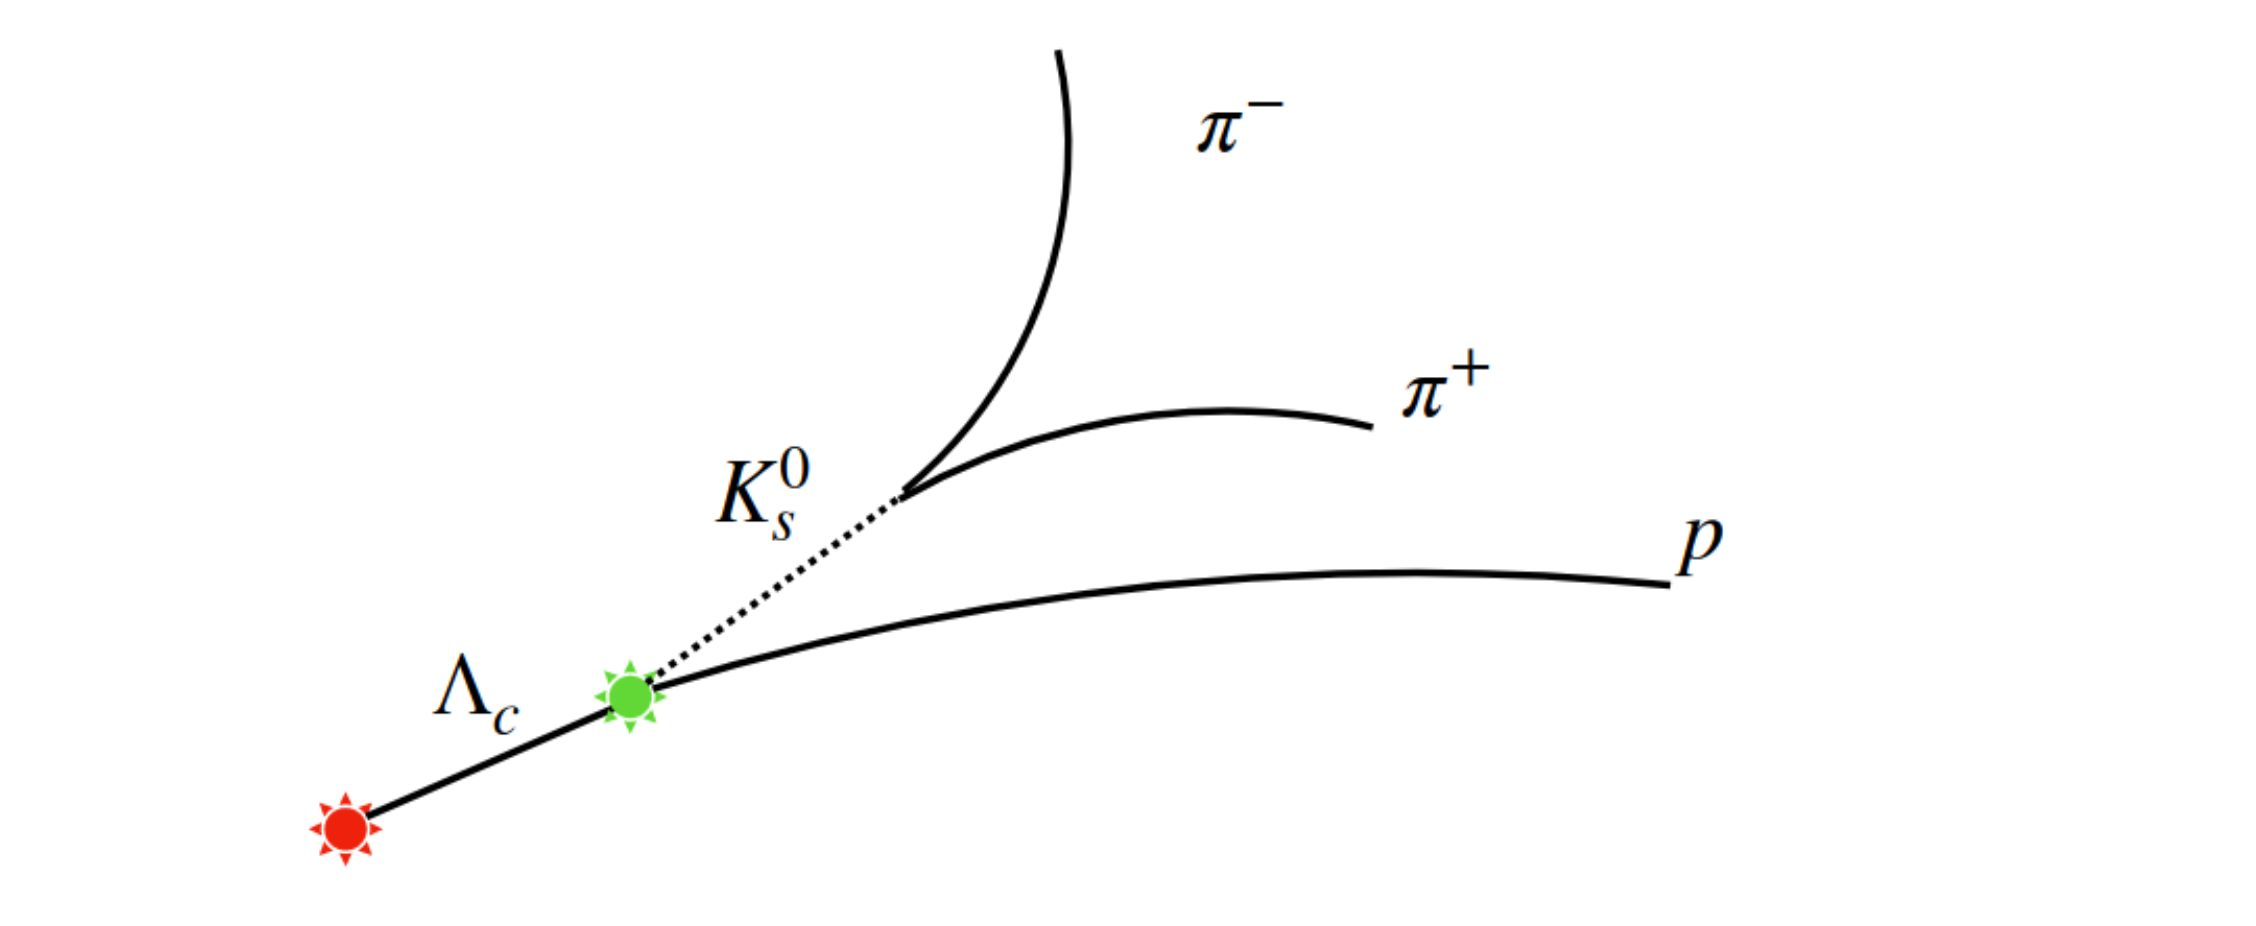
\includegraphics[width=1\linewidth]{res/fig/3-chapter/1-Lambda+c-decay.jpg}
    \caption{Rappresentazione grafica del decadimento del barione $\Lambda_{c}^{+}$ secondo il canale di decadimento $\Lambda_{c}^{+} \to p K^{0}_{S}$~\cite{Fusconi_2022}.}
    \label{fig:3-1-Lambda+c-decay}
\end{figure}
% FALLO COL PACCHETTO DEI DIAGRAMMI DI FEYMAN

I Branching Ratio (BR) di questi canali di decadimento, ovvero le \textit{probabilità} di decadimento di questi canali, sono rispettivamente:
\begin{itemize}
    \item[-] \qty[]{}{} (6.28 ± 0.32)\% per il canale~\ref{eq:3-Lambda+c-decay-channel-pKpi},

    \item[-] \qty[]{}{} (1.59 ± 0.08)\% per il canale~\ref{eq:3-Lambda+c-decay-channel-pK0S} e

    \item[-] \qty[separate-uncertainty=true]{}{} (3.60 ± 0.40)\% per il canale~\ref{eq:3-Lambda+c-decay-channel-Lambdae+nue}.
\end{itemize}

Nella presente tesi viene preso in considerazione solamente il canale di decadimento~\ref{eq:3-Lambda+c-decay-channel-pK0S} della $K^{0}_{S}$ rappresentato in
figura~\ref{fig:3-1-Lambda+c-decay}.

Il punto in cui avviene la collisione ad alta energia tra due protoni dei fasci collidenti viene detto vertice primario, nella figura rappresentato in rosso, con la conseguente+formazione del barione $\Lambda_{c}^{+}$. Conseguentemente, la $\Lambda_{c}^{+}$ decade per interazione debole, (nel punto detto vertice secondario, rappresentato in verde in figura) con le particelle figlie che sono rispettivamente un protone, il quale è stabile, e un mesone $K^{0}_{S}$ che a sua volta decade per interazione debole in due pioni carichi con un BR del (69.2 ± 0.05)\% . Sono questi ultimi due che vengono effettivamente rilevati dal rivelatore microvertice di ALICE.

La principale sfida nell’analisi di questa particella è rappresentata dalla sua brevissima vita media. Il barione $\Lambda_{c}^{+}$ ha un cτ = 60μm, e quindi in media decade dopo aver percorso una distanza inferiore alla precisione dei rivelatori di microvertice di ALICE che si attesta intorno ai 100 μm per impulsi trasversi pT ≈ 1 GeV /c. Questa situazione rende impossibile la distinzione in maniera netta tra vertice primario e vertice secondario: tale complicazione rende l’analisi considerevolmente più complessa.

Dal momento che non è possibile discriminare tra particelle provenienti dal vertice primario e quelle provenienti dal vertice secondario, è necessario implementare metodi più avanzati per separare le particelle effettivamente prodotte dal decadimento di una $\Lambda_{c}^{+}$ dal fondo (detto anche background). Questo fondo è costituito da tutte le possibili combinazioni di particelle che non derivano dal decadimento di una $\Lambda_{c}^{+}$, ma che presentano caratteristiche simili a quelle che effettivamente lo sono e che, se combinate, forniscono un valore di massa invariante accidentalmente vicino al valore della massa di una $\Lambda_{c}^{+}$.


NOOOOOOOOOOOOOOOOO%%%%%%%%%%%%%%%%%%%
A tale scopo, risulta particolarmente utile l’utilizzo di tecniche di analisi multivariata basate sul Machine Learning. In questo studio, è stato impiegato un approccio di analisi multivariata offerto dal pacchetto TMVA, come descritto nel capitolo 4.

\section{}